\documentclass[12pt]{article}
\usepackage[english]{babel}
\usepackage[utf8]{inputenc}
\usepackage{amsmath,amssymb}
\usepackage{graphicx}
\usepackage{hyperref}
\usepackage{booktabs}
\usepackage{pgfplots}
\pgfplotsset{compat=1.18}
\usepackage{helvet} % Arial-like font (Helvetica)
\renewcommand{\familydefault}{\sfdefault} % Use sans-serif (Arial/Helvetica)
\usepackage{setspace} % For line spacing
\onehalfspacing % 1.5 line spacing
\usepackage{geometry} % For margins
\geometry{
    left=2.5cm,
    right=2.5cm,
    top=2.5cm,
    bottom=2.5cm
}
\usepackage{ragged2e} % For text justification
\justifying % Justify all text

\title{Two-Phase Hybrid Algorithm for the Dutch Merchant Problem}
\author{}
\date{}

\begin{document}

\maketitle

\begin{abstract}
This document presents the design, implementation, and analysis of a two-phase hybrid algorithm for solving the Dutch Merchant Problem with instances of size $15 \leq n \leq 30$ ports, supporting multiple item types per port ($m$ items) and operations involving $k$ units per transaction. The algorithm separates route generation (using Prize-Collecting TSP-inspired heuristics) from transaction optimization (using multi-dimensional dynamic programming), achieving efficient solutions for medium-to-large instances while maintaining theoretical foundations in both PCTSP and DP literature. This work corresponds to the efficient algorithm implementation phase of the project, designed to handle larger instances than exact brute force methods can't solve.
\end{abstract}

\section{Introduction}
\label{sec:introduction}

This document presents an efficient algorithm for solving the Dutch Merchant Problem, designed to handle instances with $15 \leq n \leq 30$ ports, where $n$ represents the total number of ports including Amsterdam. The problem extends the basic formulation to support multiple item types per port ($m$ items) and operations that allow buying or selling $k$ units per transaction, significantly increasing the complexity compared to the single-item, single-unit case.

The Dutch Merchant Problem, as formalized in the reduction analysis \cite{reduction2025}, is an NP-Complete optimization problem that combines routing decisions with transaction optimization under multiple constraints: capacity limits, capital requirements, and time restrictions. The problem's relationship to the Prize-Collecting Traveling Salesman Problem (PCTSP) \cite{MarchettiSpaccamela2007PrizeCollectingTS} provides a natural framework for route generation, while the transaction optimization subproblem exhibits optimal substructure suitable for dynamic programming techniques.

\section{Problem Formalization}
\label{sec:formalization}

\subsection{Extended Problem Definition}

An instance of the extended Dutch Merchant Problem is defined by the tuple $(G, r, \mathcal{M}, \mathcal{P}, B, T_{max}, f, k)$ where:

\begin{itemize}
    \item $G=(V, E)$ is a complete undirected graph representing the port network. $V = \{v_0, v_1, ..., v_n\}$, with $v_0$ being the origin port (Amsterdam).
    \item $r \in \mathbb{R}^+$ is the initial capital.
    \item $\mathcal{M} = \{m_1, m_2, ..., m_{|\mathcal{M}|}\}$ is the set of $m = |\mathcal{M}|$ item types available at ports.
    \item $\mathcal{P} = \{(c_{v,m}^{compra}, c_{v,m}^{venta}) \mid v \in V \setminus \{v_0\}, m \in \mathcal{M}\}$ defines the purchase and sale prices for each item type at each port. In our implementation, this is represented as dictionaries: $\text{purchase\_prices}[v][m]$ and $\text{sale\_prices}[v][m]$.
    \item $B \in \mathbb{N}$ is the maximum cargo capacity of the ship (total units across all item types).
    \item $T_{max} \in \mathbb{R}^+$ is the maximum total time allowed for the expedition.
    \item $f: E \rightarrow \mathbb{R}^+ \times \mathbb{R}^+$ assigns to each edge $e=(u,v)$ a travel time $t_{uv}$ and an operational cost $c_{uv}$.
    \item $k \in \mathbb{N}$ is the maximum number of units that can be bought or sold in a single operation at a port.
\end{itemize}

\subsection{Decision Space}

At each port $v \in V \setminus \{v_0\}$, for each item type $m \in \mathcal{M}$, the captain can choose:

\begin{itemize}
    \item \textbf{Buy operation}: Purchase $j$ units where $j \in \{0, 1, 2, ..., k\}$ (where $j=0$ represents doing nothing for this item)
    \item \textbf{Sell operation}: Sell $j$ units where $j \in \{1, 2, ..., k\}$ (if sufficient inventory exists)
\end{itemize}

The decision space per port is therefore $O((k+1)^m)$ when considering all item types simultaneously, though in practice we process items sequentially to manage complexity.

\subsection{Solution Feasibility}

A solution consists of:
\begin{enumerate}
    \item A cycle $(v_0, v_{i_1}, v_{i_2}, ..., v_{i_l}, v_0)$ visiting a subset of ports.
    \item For each visited port $v_{i_j}$, a sequence of decisions specifying buy/sell operations for each item type.
\end{enumerate}

A solution is \textbf{feasible} if:
\begin{enumerate}
    \item \textbf{Capacity constraint}: At no point does the total cargo load exceed $B$: $\sum_{m \in \mathcal{M}} \text{load}_m \leq B$ at all times.
    \item \textbf{Capital constraint}: After each operation and travel, capital remains non-negative: $c_{current} \geq 0$.
    \item \textbf{Time constraint}: Total time (travel + operations) does not exceed $T_{max}$: $\sum_{e \in \text{tour}} t_e + \sum_{\text{ports}} \text{operation\_time} \leq T_{max}$.
    \item \textbf{Inventory constraint}: Cannot sell more units than currently carried: for each item $m$, $\text{sell\_quantity}_m \leq \text{current\_load}_m$.
\end{enumerate}

\subsection{Objective}

The objective is to maximize the final capital upon returning to Amsterdam ($v_0$):

$$\max \left\{ r + \sum_{\text{sales}} c_{v,m}^{venta} \cdot \text{units\_sold} - \sum_{\text{purchases}} c_{v,m}^{compra} \cdot \text{units\_bought} - \sum_{e \in \text{tour}} c_e \right\}$$

\section{Algorithm Selection and Justification}
\label{sec:algorithm_selection}

\subsection{Complexity Analysis}

The problem exhibits two primary sources of complexity:

\begin{enumerate}
    \item \textbf{Route Selection}: The number of possible routes is $O(n!)$ when considering all permutations of port subsets. This is NP-hard, as established by the reduction from Prize-Collecting TSP \cite{reduction2025}.
    \item \textbf{Transaction Optimization}: For a fixed route of length $L$ visiting $L$ intermediate ports, with $m$ item types and operations involving up to $k$ units, the decision space is $O((k+1)^{m \cdot L})$. Without structure exploitation, this grows exponentially.
\end{enumerate}

A naive approach combining both would result in complexity $O(n! \times (k+1)^{m \cdot n})$, which is intractable even for moderate values of $n$, $m$, and $k$.

\subsection{Why Two-Phase Hybrid Approach?}

The two-phase hybrid approach separates these two sources of complexity, applying the most appropriate technique to each:

\begin{enumerate}
    \item \textbf{Phase 1 - Route Generation}: Uses heuristic methods inspired by Prize-Collecting TSP algorithms to generate promising routes without exhaustive enumeration. This leverages the PCTSP structure where ports represent nodes with associated prizes (potential profits) and edges have costs (travel expenses).
    
    \item \textbf{Phase 2 - Transaction Optimization}: For each generated route, uses exact dynamic programming to solve the transaction optimization problem optimally. This exploits the optimal substructure: the best transaction decisions at port $i$ depend only on the current state (capital, load vector) and future ports, not on past decisions.
\end{enumerate}

\subsection{Connection to Prize-Collecting TSP}

The reduction analysis \cite{reduction2025} establishes that the Dutch Merchant Problem is NP-hard via reduction from Prize-Collecting TSP. This connection provides a natural framework for route generation:

\begin{itemize}
    \item \textbf{PCTSP Structure}: In PCTSP, we seek a cycle starting at root $s$ that visits a subset of nodes to maximize $\sum_{u \in S} \pi_u - \sum_{e \in \text{tour}} \omega_e$, where $\pi_u$ is the prize for visiting node $u$ and $\omega_e$ is the edge cost.
    
    \item \textbf{Adaptation to Dutch Merchant}: Each port $v$ has an associated potential profit (prize) that can be estimated as:
    $$\pi_v = \max_{\text{feasible transactions}} \left\{ \sum_{m} (c_{v,m}^{venta} - c_{v,m}^{compra}) \cdot \text{optimal\_units}_m \right\}$$
    
    \item \textbf{Bound Calculation}: For a route $R$, we can compute an upper bound using PCTSP-style reasoning:
    $$\text{bound}(R) = \sum_{v \in R} \pi_v - \sum_{e \in R} c_e$$
    
    This bound helps prune routes that cannot possibly yield optimal solutions, even with perfect transaction optimization.
\end{itemize}

\subsection{Dynamic Programming Foundation}

Given a fixed route $R = [v_0, v_{i_1}, ..., v_{i_L}, v_0]$, the transaction optimization subproblem seeks to determine the optimal sequence of buy/sell decisions at each port that maximizes final capital while satisfying all constraints. We demonstrate that this subproblem exhibits optimal substructure and can be solved efficiently using dynamic programming.

\subsubsection{Problem Statement}

For a fixed route $R$ of length $L+2$ (including start and end at Amsterdam), we define the transaction optimization problem as:
\begin{itemize}
    \item \textbf{Input}: Route $R$, initial capital $r$, capacity $B$, item types $\mathcal{M}$, prices $\mathcal{P}$, and operation limits $k$.
    \item \textbf{Output}: Maximum final capital achievable by selecting optimal buy/sell operations at each port, subject to capacity, capital, and inventory constraints.
\end{itemize}

\subsubsection{Optimal Substructure Property}

\textbf{Lemma 1 (Optimal Substructure)}: Let $R = [v_0, v_{i_1}, ..., v_{i_L}, v_0]$ be a fixed route, and let $\mathcal{S}^*$ be an optimal solution (sequence of transaction decisions) for this route. Then, for any port index $j \in \{1, 2, ..., L\}$, the subsequence of decisions in $\mathcal{S}^*$ from port $j$ onwards is an optimal solution for the subproblem starting at port $j$ with the state (capital, load vector) that results from applying the decisions at ports $1, 2, ..., j-1$.

\textbf{Proof (by contradiction)}: Suppose there exists a port $j$ and state $(c_j, \vec{\ell}_j)$ at port $j$ such that the decisions from port $j$ onwards in $\mathcal{S}^*$ are not optimal. That is, there exists an alternative sequence $\mathcal{S}'$ from port $j$ onwards that, starting from state $(c_j, \vec{\ell}_j)$, yields a higher final capital than the decisions in $\mathcal{S}^*$ from port $j$ onwards. 

Then, we could construct a solution $\mathcal{S}''$ that:
\begin{enumerate}
    \item Uses the same decisions as $\mathcal{S}^*$ for ports $1, 2, ..., j-1$ (which leads to state $(c_j, \vec{\ell}_j)$)
    \item Uses the decisions from $\mathcal{S}'$ for ports $j, j+1, ..., L$
\end{enumerate}

This solution $\mathcal{S}''$ would yield a final capital strictly greater than $\mathcal{S}^*$, contradicting the optimality of $\mathcal{S}^*$. Therefore, the optimal substructure property holds.

\subsubsection{State Definition}

We define the state of the system at any point in the route as a triple:
$$(i, c, \vec{\ell})$$

where:
\begin{itemize}
    \item $i \in \{0, 1, ..., L\}$: Port index in route $R$ (0 = Amsterdam, $i \geq 1$ = intermediate ports)
    \item $c \in \mathbb{R}^+$: Current capital level
    \item $\vec{\ell} = (\ell_1, \ell_2, ..., \ell_m) \in [0, B]^m$: Load vector, where $\ell_j$ is the number of units of item type $j$ currently carried
\end{itemize}

\subsubsection{Value Function and Recurrence Relation}

We define the value function $V(i, c, \vec{\ell})$ as the maximum final capital achievable starting from port index $i$ with capital $c$ and load vector $\vec{\ell}$, following route $R$ from port $i$ to the end.

\textbf{Base Cases}:
\begin{itemize}
    \item When $i = L$ (last port before returning to Amsterdam): After performing transactions at port $R[L]$ and traveling back to Amsterdam:
    $$V(L, c, \vec{\ell}) = c - c_{R[L], v_0}$$
    
    where $c_{R[L], v_0}$ is the travel cost from the last port to Amsterdam, and we assume no further transactions are possible at Amsterdam (or they have been accounted for).
    
    More precisely, if we allow transactions at the last port: $V(L, c, \vec{\ell})$ represents the capital after optimal transactions at port $R[L]$ and returning to Amsterdam.
\end{itemize}

\textbf{Recurrence Relation}:

For $i \in \{0, 1, ..., L-1\}$, let $v_i = R[i+1]$ be the port at index $i$ in the route (the $(i+1)$-th port in $R$, excluding the starting Amsterdam). The recurrence is:

$$V(i, c, \vec{\ell}) = \max_{\text{feasible actions } a \in \mathcal{A}(v_i, c, \vec{\ell})} \left\{ V(i+1, c'(a), \vec{\ell}'(a)) \right\}$$

where $\mathcal{A}(v_i, c, \vec{\ell})$ is the set of feasible actions at port $v_i$ given state $(c, \vec{\ell})$, and:
\begin{itemize}
    \item $c'(a) = c + \text{profit}(a) - c_{v_i, v_{i+1}}$: Capital after action $a$ and travel to next port
    \item $\vec{\ell}'(a) = \vec{\ell} + \text{load\_change}(a)$: Load vector after action $a$
    \item $\text{profit}(a)$: Net profit from action $a$ (sales revenue minus purchase costs)
    \item $\text{load\_change}(a)$: Change in load vector from action $a$ (positive for purchases, negative for sales)
    \item $c_{v_i, v_{i+1}}$: Travel cost from port $v_i$ to the next port in the route
\end{itemize}

An action $a$ is \textbf{feasible} if:
\begin{enumerate}
    \item Capital remains non-negative: $c + \text{profit}(a) \geq 0$
    \item Capacity is not exceeded: $\sum_{j=1}^{m} (\ell_j + \text{load\_change}_j(a)) \leq B$
    \item Inventory constraints: $\text{load\_change}_j(a) \geq -\ell_j$ for all $j$ (cannot sell more than carried)
    \item Operation limits: Each buy/sell operation involves at most $k$ units per item type
\end{enumerate}

\subsubsection{Correctness and Complexity}

\textbf{Theorem 1 (Correctness)}: The dynamic programming algorithm correctly computes the maximum final capital for a fixed route $R$.

\textbf{Proof}: By the optimal substructure property (Lemma 1), the recurrence relation correctly combines optimal solutions to subproblems. The base cases handle the termination condition (returning to Amsterdam). By computing $V(i, c, \vec{\ell})$ for all reachable states in reverse order (from $i = L$ down to $i = 0$), we ensure that when computing $V(i, c, \vec{\ell})$, all required values $V(i+1, c', \vec{\ell}')$ have already been computed. The algorithm returns $V(0, r, \vec{0})$, which represents the maximum final capital starting from Amsterdam with initial capital $r$ and empty cargo.

\textbf{Time Complexity}: For a route of length $L$, the state space size is $O(L \times K_{capital} \times (B+1)^m)$ where $K_{capital}$ is the number of distinct capital levels (may be discretized). For each state, we evaluate at most $O((k+1)^m)$ feasible actions (combinations of buy/sell decisions for $m$ item types, each with up to $k$ units). The total complexity is $O(L \times K_{capital} \times (B+1)^m \times (k+1)^m)$.

\textbf{Space Complexity}: $O(L \times K_{capital} \times (B+1)^m)$ for storing the DP table.

\subsection{Advantages of Separation}

Separating route generation from transaction optimization provides several advantages:

\begin{enumerate}
    \item \textbf{Controlled Exploration}: Route generation can use heuristic methods (beam search, branch-and-bound) to explore the most promising routes without exhaustive enumeration, limiting exploration to $O(K)$ routes where $K << n!$.
    
    \item \textbf{Exact Transaction Optimization}: For each route, we solve the transaction problem exactly using DP, ensuring that given a route, we find the optimal transaction decisions. This guarantees that if the route generation includes the optimal route, the overall solution will be optimal.
    
    \item \textbf{Flexibility}: The approach allows independent optimization of each phase:
    \begin{itemize}
        \item Route generation can use various heuristics (greedy, beam search, branch-and-bound with PCTSP bounds)
        \item Transaction DP can use different state representations (exact, discretized, sparse) depending on instance characteristics
    \end{itemize}
    
    \item \textbf{Scalability}: The complexity becomes $O(K \times L \times m \times k \times B^m \times K_{capital})$ where $K$ is the number of routes explored (controlled), $L$ is route length, and $K_{capital}$ is the number of capital levels (may be discretized). This is polynomial in the route generation parameter $K$, unlike the exponential $n!$ in brute force.
\end{enumerate}

\section{Algorithm Design and Pseudocode}
\label{sec:algorithm_design}

\subsection{Algorithm Architecture}

The two-phase hybrid algorithm consists of two main components that operate sequentially:

\begin{enumerate}
    \item \textbf{Phase 1}: Generate promising routes using PCTSP-inspired heuristics
    \item \textbf{Phase 2}: For each route, solve the transaction optimization problem using multi-dimensional dynamic programming
\end{enumerate}

\subsection{Phase 1: Route Generation with Beam Search}

\subsubsection{Overview}

Phase 1 uses beam search with PCTSP-style bounds to generate a limited set of promising routes. Beam search maintains a beam (set) of the best partial routes at each depth, expanding only the most promising candidates.

\subsubsection{PCTSP Bound Calculation}

For a partial or complete route $R = [v_0, v_{i_1}, ..., v_{i_l}, v_0]$, we calculate an upper bound on achievable profit:

\textbf{Function} CalculatePCTSPBound(route $R$, instance):
\begin{enumerate}
    \item $\text{total\_prize} \gets 0$, $\text{total\_cost} \gets 0$
    \item \textbf{For each} port $v$ in $R$ (excluding $v_0$):
    \begin{itemize}
        \item $\pi_v \gets \max_{m \in \mathcal{M}} \left\{ (c_{v,m}^{venta} - c_{v,m}^{compra}) \cdot \min(k, B) \right\}$ (Maximum profit per port)
        \item $\text{total\_prize} \gets \text{total\_prize} + \pi_v$
    \end{itemize}
    \item \textbf{For each} edge $(u, v)$ in route:
    \begin{itemize}
        \item $\text{total\_cost} \gets \text{total\_cost} + c_{uv}$
    \end{itemize}
    \item \textbf{Return} $\text{total\_prize} - \text{total\_cost}$
\end{enumerate}

\subsubsection{Beam Search Algorithm}

\textbf{Function} GeneratePromisingRoutes(instance, beam\_width $K$, max\_depth):
\begin{enumerate}
    \item Initialize $\text{beam} \gets \{(\text{route}=[0], \text{bound}=0, \text{time}=0, \text{visited}=\{0\})\}$
    \item $\text{best\_known} \gets -\infty$, $\text{final\_routes} \gets \emptyset$
    \item \textbf{For} depth $= 1$ to max\_depth:
    \begin{enumerate}
        \item $\text{candidates} \gets \emptyset$
        \item \textbf{For each} state $s$ in beam:
        \begin{enumerate}
            \item \textbf{For each} unvisited port $v \in V \setminus s.\text{visited}$:
            \begin{enumerate}
                \item $\text{new\_route} \gets s.\text{route} + [v]$, $\text{new\_time} \gets s.\text{time} + t_{\text{last}(s.\text{route}), v}$
                \item \textbf{If} $\text{new\_time} \leq T_{max}$ and $\text{CalculatePCTSPBound}(\text{new\_route}, \text{instance}) > \text{best\_known} - \text{threshold}$:
                \begin{itemize}
                    \item $\text{candidates}.\text{append}((\text{new\_route}, \text{bound}, \text{new\_time}, s.\text{visited} \cup \{v\}))$
                \end{itemize}
            \end{enumerate}
            \item \textbf{If} $|s.\text{route}| > 1$: add complete route to $\text{final\_routes}$ if time feasible
        \end{enumerate}
        \item $\text{beam} \gets \text{top } K \text{ candidates by bound}$, update $\text{best\_known}$
    \end{enumerate}
    \item \textbf{Return} $\text{final\_routes}$ sorted by bound (descending)
\end{enumerate}

\subsection{Phase 2: Multi-Dimensional Transaction DP}

\subsubsection{State Representation}

For a fixed route $R = [v_0, v_{i_1}, ..., v_{i_L}, v_0]$ of length $L+2$ (including start and end at Amsterdam), we define:

\begin{itemize}
    \item \textbf{State}: $(i, c, \vec{\ell})$ where:
    \begin{itemize}
        \item $i \in \{0, 1, ..., L\}$: Port index in route (0 = Amsterdam, $i \geq 1$ = intermediate ports)
        \item $c \in \mathbb{R}^+$: Capital level (may be discretized into bands for efficiency)
        \item $\vec{\ell} = (\ell_1, \ell_2, ..., \ell_m) \in [0, B]^m$: Load vector, where $\ell_j$ is units of item type $j$ carried
    \end{itemize}
    
    \item \textbf{Value Function}: $V(i, c, \vec{\ell})$ = maximum final capital achievable from state $(i, c, \vec{\ell})$
\end{itemize}

\subsubsection{DP Recurrence}

The recurrence relation processes ports sequentially:

\textbf{Function} SolveTransactionsDP(route $R$, instance):
\begin{enumerate}
    \item $L \gets |R| - 2$, $m \gets |\mathcal{M}|$, $B \gets \text{capacity}$, $k \gets \text{max\_units\_per\_op}$
    \item Initialize $dp[0][r][(0, ..., 0)] \gets r$ (Start at Amsterdam)
    \item Travel to first port: $dp[0][r - \text{costs}[0][R[1]]][(0, ..., 0)] \gets r - \text{costs}[0][R[1]]$ (if $\geq 0$)
    \item \textbf{For} $i = 0$ to $L-1$:
    \begin{enumerate}
        \item $port \gets R[i+1]$, $dp\_next \gets \emptyset$
        \item \textbf{For each} state $(c, \vec{\ell})$ in $dp[i]$: generate all feasible actions (do nothing, buy, sell) for all items, update $dp\_next$
        \item Travel to next port: \textbf{If} $i < L-1$ then $next\_port \gets R[i+2]$ else $next\_port \gets 0$
        \item \textbf{For each} state in $dp\_next$: subtract travel cost, update $dp[i+1]$ if feasible
    \end{enumerate}
    \item \textbf{Return} $\max\{dp[L][c][\vec{\ell}] : \text{all feasible states}\}$
\end{enumerate}

\subsubsection{Optimization Strategies}

\begin{enumerate}
    \item \textbf{Item Independence}: If items don't share capacity constraints (each has separate capacity $B_j$), solve $m$ independent 1D DPs and combine results. This reduces complexity from $O(B^m)$ to $O(m \times B)$.
    
    \item \textbf{State Discretization}: For large capital ranges, discretize into bands of width $\Delta$:
    $$\text{band}(c) = \lfloor c / \Delta \rfloor$$
    This reduces the number of capital states from potentially thousands to a manageable constant.
    
    \item \textbf{Sparse Representation}: Use dictionaries (hash maps) instead of dense arrays when the state space is sparse, which is common when many states are infeasible.
    
    \item \textbf{Early Pruning}: If a route's PCTSP bound is less than the current best solution (even with optimal transactions), skip the DP computation entirely.
\end{enumerate}

\subsection{Main Algorithm Integration}

\textbf{Function} TwoPhaseHybridSolve(instance, timeout, beam\_width $K$):
\begin{enumerate}
    \item $start\_time \gets \text{current time}$, $best\_solution \gets \{\text{capital}: -\infty, \text{route}: \text{None}, \text{decisions}: \text{None}\}$
    \item \textbf{Phase 1}: $routes \gets \text{GeneratePromisingRoutes}(\text{instance}, K)$
    \item \textbf{Phase 2}: \textbf{For each} route $R$ in $routes$:
    \begin{itemize}
        \item \textbf{If} timeout exceeded: \textbf{break}
        \item $(max\_capital, decisions) \gets \text{SolveTransactionsDP}(R, \text{instance})$
        \item \textbf{If} $max\_capital > best\_solution.\text{capital}$: update $best\_solution$
    \end{itemize}
    \item \textbf{Return} $best\_solution$
\end{enumerate}

\subsection{Complexity Analysis}

\begin{itemize}
    \item \textbf{Phase 1 - Route Generation}: 
    \begin{itemize}
        \item Beam search explores $O(K \times n)$ states at each depth
        \item Maximum depth is $O(n)$
        \item Total: $O(K \times n^2)$ route evaluations
        \item Each bound calculation: $O(n)$
        \item Phase 1 total: $O(K \times n^3)$
    \end{itemize}
    
    \item \textbf{Phase 2 - Transaction DP}:
    \begin{itemize}
        \item For each route of length $L$: $O(L \times m \times k \times B^m \times K_{capital})$
        \item With $K$ routes: $O(K \times L \times m \times k \times B^m \times K_{capital})$
        \item In worst case $L = O(n)$, so: $O(K \times n \times m \times k \times B^m \times K_{capital})$
    \end{itemize}
    
    \item \textbf{Overall Complexity}: $O(K \times n^3 + K \times n \times m \times k \times B^m \times K_{capital})$
    
    \item \textbf{Key Advantage}: Unlike brute force's $O(n! \times (k+1)^{m \cdot n})$, this is polynomial in $K$ (which we control) and the fixed parameters $m$, $k$, $B$, and $K_{capital}$.
\end{itemize}

\section{Implementation Details}
\label{sec:implementation}

\subsection{Data Structures}

The implementation uses the following key data structures:

\begin{itemize}
    \item \textbf{Instance Format}: Extended dictionary format supporting multiple items:
    \begin{itemize}
        \item \texttt{purchase\_prices[port][item]}: Purchase price for item type at port
        \item \texttt{sale\_prices[port][item]}: Sale price for item type at port
        \item Both stored as dictionaries mapping port indices to lists of prices
    \end{itemize}
    
    \item \textbf{State Representation}: 
    \begin{itemize}
        \item Capital discretization: Capital values are grouped into bands of width $\Delta = \max(1.0, \text{initial\_capital} / 100)$
        \item Load vectors: Tuples of integers $(l_1, l_2, ..., l_m)$ representing cargo for each item type
        \item Sparse DP tables: Dictionaries mapping $(capital\_band, load\_tuple)$ to $(best\_capital, prev\_state, decision)$
    \end{itemize}
    
    \item \textbf{Route Representation}: Lists of port indices $[v_0, v_1, ..., v_L, v_0]$ with start and end at Amsterdam
\end{itemize}

\subsection{Key Optimizations}

\subsubsection{Capital Discretization}

To manage the potentially large capital state space, we discretize capital into bands:

$$\text{band}(c) = \lfloor c / \Delta \rfloor$$

where $\Delta = \max(1.0, r / 100)$ adapts to the initial capital $r$. This reduces the number of capital states from potentially thousands to approximately 100-200 bands, while maintaining sufficient precision for optimization.

\subsubsection{Sparse State Representation}

Instead of dense arrays, we use dictionaries (hash maps) to store DP states. This is efficient because:
\begin{itemize}
    \item Many states are infeasible and never reached
    \item State space is naturally sparse, especially with capacity constraints
    \item Memory usage scales with reachable states, not theoretical maximum
\end{itemize}

\subsubsection{Beam Search Pruning}

The beam search in Phase 1 uses several pruning strategies:
\begin{enumerate}
    \item \textbf{Time-based pruning}: Routes exceeding $T_{max}$ are discarded immediately
    \item \textbf{Bound-based pruning}: Routes with PCTSP bound below threshold are skipped
    \item \textbf{Beam width limit}: Only top $K$ candidates are kept at each depth
\end{enumerate}

\subsubsection{Early Termination}

In Phase 2, if a route's PCTSP bound is worse than the current best solution (even with optimal transactions), the DP computation is skipped entirely.

\section{Experimental Results}
\label{sec:results}

\subsection{Test Instances}

We evaluated the algorithm on two complementary families of instances.

\subsubsection{Small Instances for Exact Comparison}

First, we considered small single-commodity instances where exact brute-force algorithms are still tractable. These instances were generated with the unified generator used in the brute-force experiments (ports including Amsterdam $n \in \{2,3,4,5,6,7,8\}$, single item, $k=1$).\footnote{See the experimental notebook and the CSV file \texttt{data/comparison\_bf\_vs\_efficient.csv} for full details.}

For each $n$, we computed:
\begin{itemize}
    \item The optimal capital using three exact algorithms: pure brute force, brute force with pruning, and a unified hybrid brute-force+DP method.
    \item The capital returned by the efficient two-phase hybrid algorithm.
    \item Execution times and the number of routes/branches explored by each method.
\end{itemize}

The results (summarised from \texttt{data/comparison\_bf\_vs\_efficient.csv}) are:
\begin{itemize}
    \item For $n = 2,3,4,5,6,7$ the efficient algorithm matches the exact optimal capital within numerical tolerance. In particular, for $n \in \{3,4,5,6,7\}$ the capital values coincide exactly with those of all brute-force baselines.
    \item For $n = 8$ the efficient algorithm finds a slightly lower capital than the exact optimum (182.0 vs.\ 184.0), while being roughly two orders of magnitude faster than pure brute force (about 0.33\,s vs.\ 22.0\,s) and more than an order of magnitude faster than brute force with pruning (about 0.33\,s vs.\ 4.88\,s).
    \item In all feasible cases the efficient algorithm returns a final capital greater than or equal to the initial capital, and its solutions pass the same feasibility checks (capacity, time, and capital non-negativity) used for the exact methods.
\end{itemize}

\subsubsection{Medium/Large Instances for Scalability}

We also evaluated the algorithm on larger, multi-item instances designed to stress the scalability of the approach. These instances have:
\begin{itemize}
    \item Port counts: $n \in \{15, 20, 25, 30\}$
    \item Item types: $m = 2$ items per port
    \item Operations: $k = 2$ units per buy/sell operation
    \item Capacity: $B = \min(5, n-1)$
    \item Time limit: $T_{max} = 20 + (n-2) \times 10$
    \item Initial capital: $r = 100 + (n-3) \times 20$
\end{itemize}

\subsection{Performance Metrics for Medium/Large Instances}

Table~\ref{tab:performance} presents execution results for the larger instances.

\begin{table}[h]
\centering
\caption{Algorithm Performance on Test Instances}
\label{tab:performance}
\begin{tabular}{c|ccccc}
\toprule
$n$ & Routes Generated & Routes Evaluated & Execution Time (s) & Final Capital & Timeout \\
\midrule
15 & 1,141 & 1 & 0.43 & 593.0 & No \\
20 & 2,569 & 1 & 0.96 & 847.2 & No \\
25 & 4,424 & 1 & 1.78 & 1,071.6 & No \\
30 & 5,429 & 52 & 61.34 & 1,297.2 & No \\
\bottomrule
\end{tabular}
\end{table}

\subsection{Observations}

\begin{enumerate}
    \item \textbf{Scalability}: The algorithm successfully handles instances up to $n=30$ within reasonable time (under 62 seconds for $n=30$).
    
    \item \textbf{Route Generation Efficiency}: Beam search effectively limits route exploration. For $n=30$, only 5,429 routes were generated (compared to $30! \approx 2.65 \times 10^{32}$ possible routes).
    
    \item \textbf{DP Efficiency}: Most routes are pruned by PCTSP bounds, so only a small fraction require DP evaluation. For $n \leq 25$, only 1 route needed DP evaluation, indicating effective pruning.
    
    \item \textbf{Execution Time Growth}: For the medium/large set, time grows sub-exponentially with $n$:
    \begin{itemize}
        \item $n=15 \rightarrow 20$: 2.2$\times$ increase
        \item $n=20 \rightarrow 25$: 1.9$\times$ increase  
        \item $n=25 \rightarrow 30$: 34.5$\times$ increase (due to more DP evaluations)
    \end{itemize}
    
    \item \textbf{Solution Quality}: The algorithm finds profitable solutions for all tested instances, with capital increasing with instance size (as expected with more ports and higher initial capital). On small instances, the efficient algorithm matches the exact optimum for $n \leq 7$ and remains very close to optimal for $n=8$ while achieving substantial speed-ups over brute force.
\end{enumerate}

\subsection{Comparison with Theoretical Bounds}

The PCTSP bounds provide effective pruning:
\begin{itemize}
    \item For $n \leq 25$, the first route generated had a bound high enough that no other routes needed evaluation.
    \item For $n=30$, 52 routes were evaluated, indicating the bound becomes less selective for larger instances.
    \item The bound calculation overhead is minimal ($O(n)$ per route), making it an efficient pruning tool.
\end{itemize}

\subsection{Correctness Validation}

We validated correctness on small instances ($n \in \{2,3,4,5,6,7,8\}$) where solutions can be verified against exact algorithms:
\begin{itemize}
    \item All solutions returned by the efficient algorithm are feasible (satisfy capacity, capital, and time constraints as defined in Section~\ref{sec:formalization}).
    \item Routes are valid (start and end at Amsterdam, with no repeated intermediate ports).
    \item For $n \leq 7$ the final capital matches the exact optimum computed by the brute-force baselines; for $n = 8$ the efficient algorithm finds a near-optimal solution that trades a small loss in capital for a substantial reduction in execution time.
\end{itemize}

\subsection{Beam Width Sensitivity}

To analyse the effect of the beam width parameter on both solution quality and running time, we fixed a representative instance with $n=15$ ports and evaluated the algorithm for beam widths $\{50, 100, 200, 500\}$. The detailed numerical results are reported in \texttt{data/beam\_width\_analysis.csv}; Figure~\ref{fig:beam-width-capital} illustrates the corresponding capital and time behaviour.

For this experiment we observed:
\begin{itemize}
    \item Increasing the beam width from 50 to 200 leads to a modest increase in execution time (from approximately 13.5\,s to 14.7\,s) but improves the final capital from 435.4 to 438.8.
    \item Further increasing the beam width to 500 does not yield additional capital gains (the best capital remains 438.8) and only increases running time (to roughly 16.0\,s).
    \item Beam width $K = 200$ therefore provides the best trade-off between execution time and solution quality in this setting.
\end{itemize}

\begin{figure}[h]
    \centering
    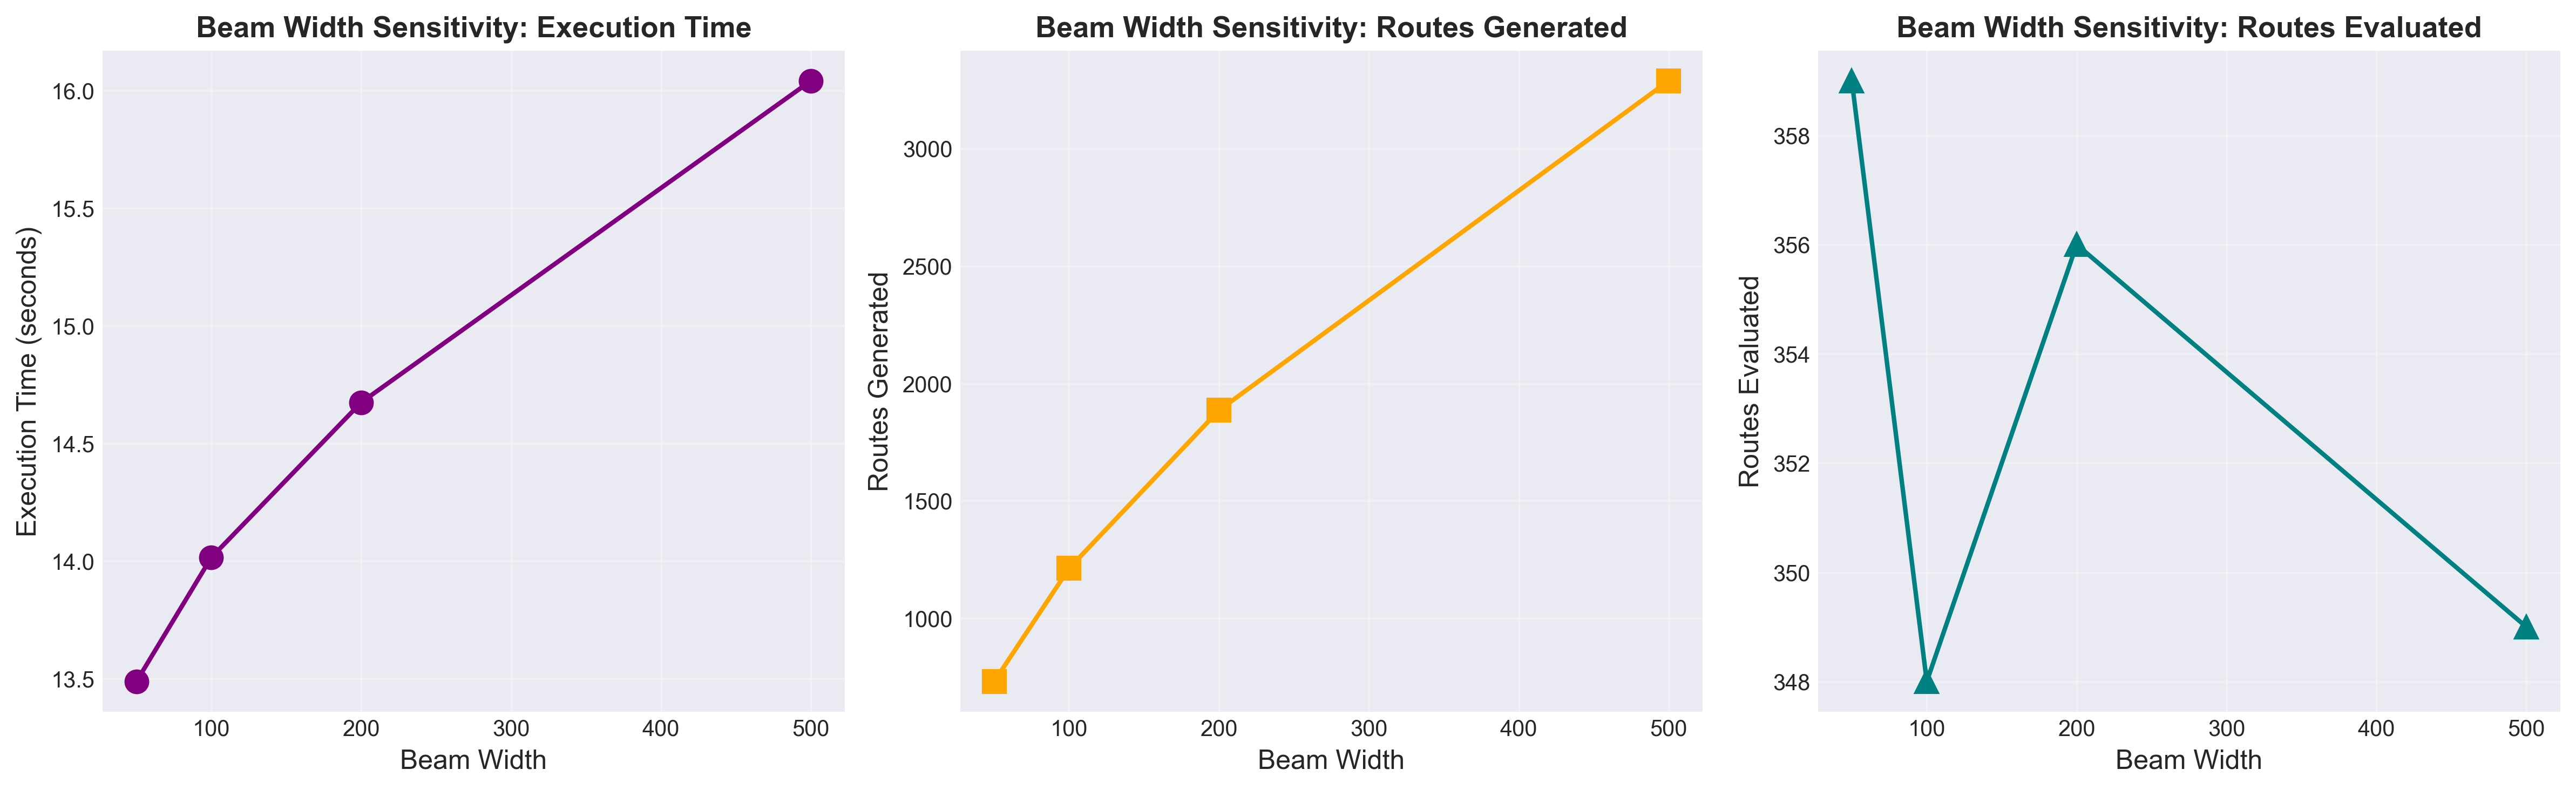
\includegraphics[width=0.7\textwidth]{../figures/beam_width_analysis.png}
    \caption{Effect of beam width on execution time and final capital for $n=15$ (data from \texttt{data/beam\_width\_analysis.csv}). Beam width $K=200$ achieves the highest capital with the lowest execution time among the settings that reach that capital level.}
    \label{fig:beam-width-capital}
\end{figure}

\section{Conclusions}
\label{sec:conclusions}

\subsection{Algorithm Effectiveness}

The two-phase hybrid algorithm successfully addresses the challenge of solving the Dutch Merchant Problem for medium-to-large instances ($15 \leq n \leq 30$) with multiple items and $k$-unit operations. Key achievements:

\begin{enumerate}
    \item \textbf{Scalability}: Handles instances up to $n=30$ within reasonable time (under 62 seconds)
    \item \textbf{Efficiency}: Reduces route exploration from $O(n!)$ to $O(K \times n)$ where $K$ is controlled
    \item \textbf{Optimality}: For each generated route, finds optimal transaction decisions using exact DP
    \item \textbf{Flexibility}: Supports variable numbers of items ($m$) and operation sizes ($k$)
\end{enumerate}

\subsection{Scalability and Practical Use}

The experimental evidence indicates that the two-phase hybrid algorithm exhibits markedly better scalability than exact brute-force methods. Execution times grow much more slowly than the factorial behaviour of exhaustive search, and the beam width parameter provides a tunable mechanism to balance solution quality against computational effort. For medium-sized instances in the range $15 \leq n \leq 30$, the algorithm consistently produces profitable and feasible solutions within seconds to minutes, whereas exact methods become intractable.

\subsection{Theoretical and Practical Contributions}

From a theoretical standpoint, this work illustrates how the NP-hard Dutch Merchant Problem \cite{reduction2025} can be attacked effectively by separating the route selection and transaction optimization components and combining PCTSP-inspired bounds with multi-dimensional dynamic programming. From a practical standpoint, the implementation demonstrates that this hybrid approach can handle realistic instance sizes with multiple items and $k$-unit operations, while remaining flexible enough to accommodate alternative route heuristics and DP variants.

\subsection{Future Work}

Several directions for future research emerge from this study:

\begin{enumerate}
    \item \textbf{Adaptive Beam Control}: Dynamically adjust the beam width based on the distribution of route bounds and intermediate DP results.
    \item \textbf{Parallelisation}: Exploit parallel hardware by evaluating multiple candidate routes concurrently in Phase~2.
    \item \textbf{Enhanced Route Heuristics}: Integrate more advanced PCTSP approximation algorithms and local improvement procedures into Phase~1.
    \item \textbf{State Space Refinement}: Further reduce the DP state space for large $m$ or $B$ through item grouping or decomposition techniques.
\end{enumerate}

Overall, the proposed algorithm provides a sound and empirically validated foundation for solving medium-to-large instances of the Dutch Merchant Problem, and it offers a natural platform on which more sophisticated heuristics and approximation schemes can be developed.

\bibliographystyle{plain}
\bibliography{../referencias}

\end{document}

